\section{Numerical Integration}

\begin{wrapfigure}{l}{0.15\textwidth}
  \begin{center}
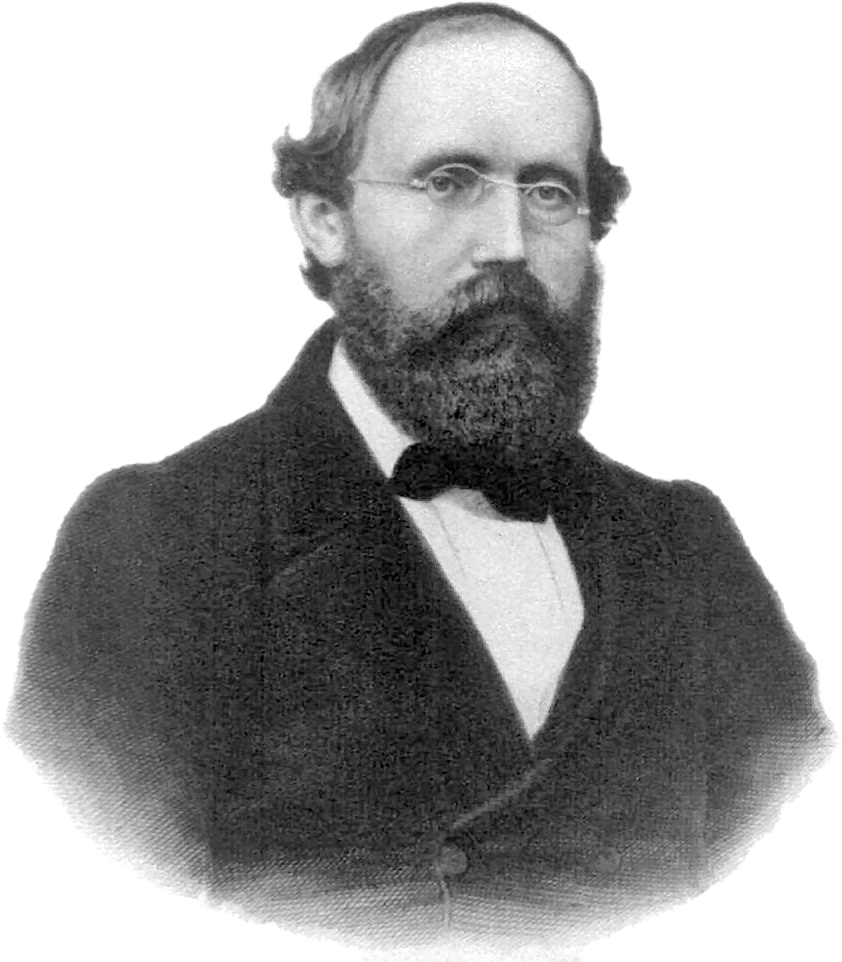
\includegraphics[width=0.15\textwidth]{images/riemann.png} \\
\emph{B.\xspace Riemann}
  \end{center}
\end{wrapfigure}

A Riemann sum (Bernhard Riemann, 17 September 1826--20 July 1866) is an
approximation of a definite integral by a finite sum. The sum is calculated by
partitioning the region into shapes (rectangles, trapezoids, parabolas, or
cubics) that together form a region that is similar to the region being
measured, then calculating the area for each of these shapes, and finally
summing these small areas. This approach can be used to find a numerical
approximation for a definite integral even if the fundamental theorem of
calculus does not make it easy to find a closed-form solution.

Because the region filled by the small shapes is usually not exactly the
same shape as the region being measured, the Riemann sum will differ
from the area being measured. This error can be reduced by dividing up
the region more finely, using smaller and smaller shapes. As the shapes
decrease in size, the sum approaches the value of the integral.

The left Riemann sum approximates $f$ by its value at the
left-end point gives multiple rectangles with base $\Delta x$ and height
$f(a + i\Delta x)$. Doing this for $i = 0, 1, \ldots , n-1$, and summing
the resulting areas gives
$$
A_\text{left} =
\Delta x \left[f(a) + f(a + \Delta x) + f(a+ 2 \, \Delta x)+ \cdots+f(b - \Delta x)\right].
$$
The left Riemann sum overestimates if $f$ is
\emph{monotonically decreasing} on this interval, and underestimates
if it is \emph{monotonically increasing}.

The right Riemann sum approximates $f$ by its value at the
right end-point. This gives
multiple rectangles with base $\Delta x$ and height $f(a + i\Delta x)$.
Doing this for $i = 1, \ldots, n$, and summing the resulting areas
produces
$$
A_\text{right} = \Delta x \left[ f( a
+ \Delta x ) + f(a + 2 \, \Delta x)+\cdots+f(b) \right].
$$
The right Riemann sum underestimates if $f$ is
monotonically decreasing, and overestimates if it is monotonically
increasing.

The \emph{midpoint rule} approximates $f$ at the midpoint of intervals, giving
$f(a + \tfrac{\Delta x}{2})$ for the first interval, for the next one
$f(a + 3\tfrac{\Delta x}{2})$, and so on until $f(b-\tfrac{\Delta
x}{2})$. Summing up the areas gives
$$
A_\text{mid} = \Delta x\left[f \left(a +
\tfrac{\Delta x}{2} \right) + f \left(a + \tfrac{3\,\Delta x}{2}
\right) + \cdots+f \left(b-\tfrac{\Delta x}{2} \right)\right].
$$

Refer to Figures \ref{figure:riemann-sin} and \ref{figure:riemann-cos}
for example plots of Riemann sums.

\begin{figure}[bth]
  \begin{centering}
    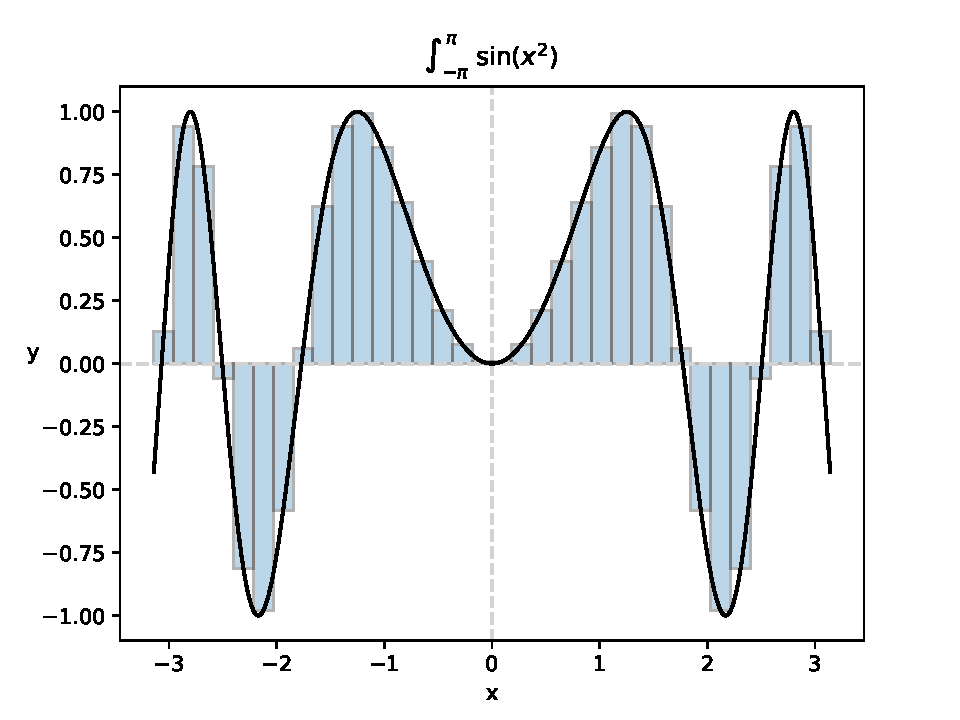
\includegraphics[width=0.65\textwidth]{riemann/sin.pdf}
    \caption{Midpoint Riemann sum for $\sin(x^2)$ over the range $[-\pi,
    \pi]$ with 50 partitions.}\label{figure:riemann-sin}
  \end{centering}
\end{figure}

\begin{figure}[bth]
  \begin{centering}
    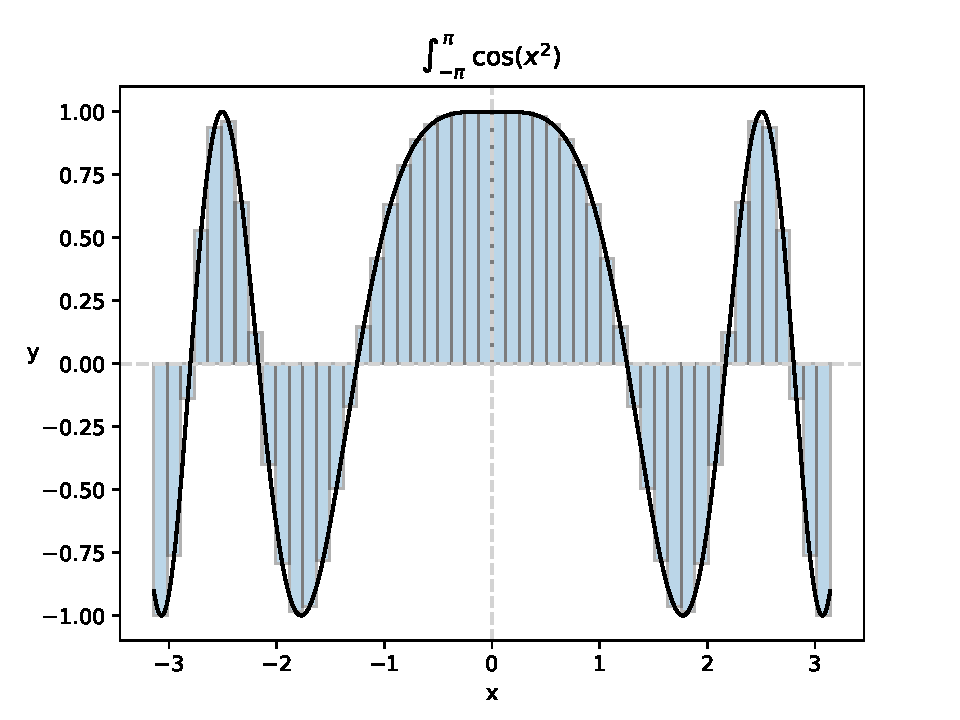
\includegraphics[width=0.65\textwidth]{riemann/cos.pdf}
    \caption{Midpoint Riemann sum for $\cos(x^2)$ over the range $[-\pi,
    \pi]$ with 50 partitions.}\label{figure:riemann-cos}
  \end{centering}
\end{figure}

\subsection{The Trapezoidal Rule}

The \emph{trapezoidal rule} (also known as the \emph{trapezoid rule}) is an
example of a closed Newton-Cotes quadrature. In numerical analysis,
this is a common technique for approximating a \emph{definite integral}.

It is assumed that the value of a function $f$ defined on $[a,b]$
is known at $n+1$ equally spaced points: $a \leq x_0 < x_1 < \dots
< x_n \leq b$. It is a form of \emph{closed} Newton–Cotes quadrature where
$x_0 = a$ and $x_n = b$, using
the function values at the interval end-points.
Newton–Cotes formulas using $n+1$ points can be
defined as
$$\int_a^b f(x) \,dx \approx \sum_{i=0}^n w_i\, f(x_i)$$
where $x_i = a + i h$, with
$h = (b-a)/n$.

The number $h$ is called \emph{step size}, $w_i$ are called \emph{weights}. The
weights can be computed as the integral of Lagrange basis polynomials, but you
do not need to worry about those here. Just know that they depend only on $x_i$
and not on the function $f$.

The trapezoidal rule works by approximating the region under the graph
of the function $f(x)$ as a trapezoid and calculating its area. It
follows that
$$
\int_{a}^{b} f(x) \, dx \approx \frac{b-a}{2} \left( f(a)+f(b) \right).
$$

The trapezoidal rule may be viewed as the result obtained by averaging
the left and right Riemann sums. The
integral can be even better approximated by partitioning the integration
interval, applying the trapezoidal rule to each subinterval, and summing
the results. In practice, this \emph{composite}
trapezoidal rule is usually what is meant by ``integrating with the
trapezoidal rule.'' Let $\{x_k\}$ be a partition of $[a,b]$ such that
$a=x_0 < x_1 < \cdots < x_{n-1} < x_n = b$ and $\Delta x_k$ be the
length of the $k^\text{th}$ subinterval (that is, $\Delta x_k = x_k -
x_{k-1}$), then
$$
\int_a^b f(x) \, dx \approx \sum_{k=1}^n \frac{f(x_{k-1}) + f(x_k)}{2} \Delta x_k.
$$

When the partition has a regular spacing,
when all the $\Delta x_k$ have the same value $\Delta x,$ the formula
can be simplified for calculation efficiency by factoring $h=\Delta x$
out:
\begin{align*}
\int_a^b f(x) \, dx & \approx \frac{h}{2}
\left(f(x_0) + 2f(x_1) + 2f(x_2) + 2f(x_3) + 2f(x_4) + \cdots +
2f(x_{n-1}) + f(x_n)\right) \\
& = \frac{h}{2}
\left(f(x_0) + 2\sum_{i=1}^{n-1} f(x_i) + f(x_n)\right).
\end{align*}
As $n$ increases, $h$ decreases, and as the resolution of the
partition increases the approximation becomes more accurate.

If we assume a fixed size $h = (b - b)/n$, then it is simple to
write the code for the trapezoid rule.

\begin{pylisting}{Implementation of the trapezoidal rule}
def trapezoid(f, a, b, n):
    h = (b - a) / n
    sum = f(a) + f(b)
    for j in range(1, n):
        sum += 2.0 * f(a + j * h)
    sum *= h / 2.0
    return sum
\end{pylisting}

\subsection{Simpson's Rules}


\begin{wrapfigure}{r}{0.11\textwidth}
  \begin{center}
  
\includegraphics[width=0.10\textwidth]{images/homer.png}\\
          \emph{H.\xspace Simpson}
  \end{center}
\end{wrapfigure}
We can do better than using the simple trapezoidal rule by adopting one of
Simpson's Rules  for approximating definite
integrals. Thomas Simpson (1710--1761) was a self-taught mathematician who supported himself
during his early years as a weaver. His primary interest was probability theory,
although in 1750 he published a two-volume calculus book entitled \emph{The
Doctrine and Application of Fluxions}. In German and some other languages, the
simplest of these rules is named after Johannes Kepler, who derived it in 1615
after seeing it used for wine barrels (\emph{Keplersche Fassregel}\,). The
approximate equality in the rule becomes exact if $f$ is a polynomial up to
$3^\text{rd}$ degree.

Interpolation with polynomials evaluated at equally spaced points in $[a,b]$
yields a Newton–Cotes formulas, of which the \emph{rectangle rule} and the
\emph{trapezoidal rule} are examples. Simpson's rule, which is based on a
polynomial of order 2, is also a Newton–Cotes formula.

\subsubsection{Simpson's 1/3 Rule}

Simpson's 1/3 rule is also an instance of a Newton-Cotes quadrature formula.
If the interval of integration $[a, b]$ is in some sense \emph{small},
then Simpson's rule with $n = 2$ subintervals will provide an
adequate approximation to the exact integral. By small we mean that
the function being integrated is relatively smooth over the interval
$[a, b]$. For such a function, a smooth quadratic interpolant like
the one used in Simpson's rule will give good results:

$$
\int_a^b f(x) \, dx \approx \frac{b - a}{6} \left[f(a) + 4f\left(\frac{a + b}{2}\right) + f(b)\right].
$$

\subsubsection{Composite Simpson's 1/3 Rule}\label{section:compositesimpson}

It is often the case that the function we are trying to integrate is not smooth
over the interval. Typically, this means that either the function is highly
oscillatory or lacks derivatives at certain points. One common way of handling
this problem is by breaking up the interval $[a, b]$ into $n > 2$ small
subintervals. Simpson's rule is then applied to each subinterval, with the
results being summed to produce an approximation for the integral over the
entire interval. This approach is termed the \emph{Composite Simpson's 1/3
rule}.

Suppose that the interval $[a, b]$ is split up into $n$ sub-intervals,
with $n$ an even number. Then, the composite Simpson's 1/3 rule is given by
\begin{align*}
  \int_a^b f(x) \, dx &\approx \frac{h}{3}
   \sum_{j=1}^{n/2}\big[f(x_{2j-2}) + 4f(x_{2j-1}) + f(x_{2j})\big] \\
  &= \frac{h}{3}
   \bigg[f(x_0) + 2\sum_{j=1}^{n/2-1} f(x_{2j}) + 4\sum_{j=1}^{n/2} f(x_{2j-1}) + f(x_n)\bigg],
 \end{align*}
where $x_j = a + jh$ for $j = 0, 1, \dots, n - 1, n$ with $h = (b -
a)/n$; in particular, $x_0 = a$ and $x_n = b$. The error when using the
composite Simpson's 1/3 rule is
$$
-\frac{h^4}{180} (b - a)f^{(4)}(\xi),
$$
where $\xi$ is some number between $a$ and $b$, and $h = (b - a)/n$ is
the step length.

\subsection{High Order Formul\ae}

These are not the only closed Newton-Cotes quadratures used for
numerical integration. For example, there is the composite Simpson's 3/8 rule:
 \begin{align*}
  \int_a^b f(x) \, dx &\approx \frac{3h}{8} \big[f(x_0) + 3f(x_1) + 3f(x_2) + 2f(x_3) + 3f(x_4) + 3f(x_5) + 2f(x_6) + {} \\
  &\qquad\qquad \cdots + 3f(x_{n-2}) + 3f(x_{n-1}) + f(x_n)\big] \\
  &= \frac{3h}{8} \left[f(x_0) + 3 \sum_{i \ne 3k}^{n-1} f(x_i) + 2 \sum_{j=1}^{n/3 - 1} f(x_{3j}) + f(x_n) \right] \quad \text{for  } k \in \mathbb{N}_0.
 \end{align*}
It has a smaller error term of
$$
 -\frac{h^4}{80} (b - a)f^{(4)}(\xi),
$$
but can only be used  this if $n$ is a \emph{multiple of three}.

Simpson's 3/8 rule is more difficult to implement directly, since it is not
obvious how we write a loop for the first summation. Instead, we ask what that
summation actually means: it means sum for all indices that are not multiples of
$3$ and the second summation for multiples of $3$. The code then follows easily.

\begin{pylisting}{Implementation of composite Simpson's 3/8 rule}
def simpson_38(f, a, b, n):
    h = (b - a) / n
    sum = f(a) + f(b)
    for i in range(1, n):
        if i % 3 != 0:
            sum += 3 * f(a + i * h)
        else:
            sum += 2 * f(a + i * h)
    sum *= h * 3 / 8
    return sum
\end{pylisting}

And, finally, there is the composite Boole's rule.
Yes, that George Boole (2 November 1815--8 December 1864), the founder of Boolean logic.
Boole's rule is also a Newton-Cotes formula with a decreased error term. In order to use Boole's composite rule, the number of partitions should be a multiple of 12.
$$
  \int_{a}^{b} f(x)\,dx
  = \frac{2 h}{45}
    \left(
         7(f(x_0) + f(x_n))
      + 32\left(\sum_{i \in \{1, 3,  \ldots, n-1\}} f(x_i)\right)
      + 12\left(\sum_{i \in \{2, 6,  \ldots, n-2\}} f(x_i)\right)
      + 14\left(\sum_{i \in \{4, 8,  \ldots, n-4\}} f(x_i)\right)
    \right)
$$
that has the error term
$$
-\,\frac{8}{945} h^7 f^{(6)}(\xi) .
$$

The formula for Boole's rule might appear daunting, but the code is not too bad.
It just requires a little thought. Again, you ask, ``What does each summation
do?''

\begin{pylisting}{Implementation of Boole's rule}
def boole(f, a, b, n):
    h = (b - a) / n
    sum = 7 * (f(a) + f(b))
    for i in range(1, n, 2):     sum += 32 * f(a + i * h)
    for i in range(2, n - 1, 4): sum += 12 * f(a + i * h)
    for i in range(4, n - 3, 4): sum += 14 * f(a + i * h)
    sum *= h * 2 / 45
    return sum
\end{pylisting}

If you are intrigued by these and other numerical computations, then we
encourage you to do some reading on you own, or take a course in the Applied
Mathematics department.

\begin{itemize}
  \item Burden, Richard L., and J. Douglas Faires. \emph{Numerical Analysis},
  $7^\text{th}$ edition, 2001. Thomson Learning ISBN 0-534-38216-9.
  \item Abramowitz, Milton, and Irene A. Stegun, \emph{eds}. \emph{Handbook of
    mathematical functions with formulas, graphs, and mathematical tables}. Vol.
    55. US Government printing office, 1970.
\end{itemize}
